\documentclass[10pt]{article}


\usepackage[utf8]{inputenc}
\usepackage[T1]{fontenc}
\usepackage[frenchb]{babel}

\usepackage{algorithm}
\usepackage{algorithmic}
\usepackage[T1]{fontenc}
\usepackage{enumitem}
\usepackage{hyperref}
\usepackage{graphicx}
\usepackage{color}
\usepackage{listings}
\usepackage{wrapfig}
\usepackage{amsfonts}
\usepackage{amsmath}
\usepackage{mathtools}
\usepackage[hmargin=1.25in,vmargin=1.25in]{geometry}
\usepackage{framed}
\usepackage{mathenv}
\usepackage{blkarray}

%title setuplisting
\title{Projet WEB de groupe}
\author{
  Gangyue CHEN \\
  Louis LAFUMA \\
  Baptiste LAMBERT \\
  Romain PEREIRA
}
\date{22/05/2018}

% table of contents setup
\renewcommand{\contentsname}{Sommaire}
\usepackage{etoolbox}
\patchcmd{\thebibliography}{\section*{\refname}}{}{}{}

\setlength{\parindent}{0cm}
\setlength{\parskip}{1ex plus 0.5ex minus 0.2ex}
\newcommand{\hsp}{\hspace{20pt}}
\newcommand{\HRule}{\rule{\linewidth}{0.5mm}}

\hypersetup{
  colorlinks,
  citecolor=black,
  filecolor=black,
  linkcolor=blue,
  urlcolor=red
}

\begin{document}
  \begin{titlepage}
    \begin{sffamily}
      \begin{center}
	
	\textsc{\LARGE ENSIIE}\\[2cm]
	\textsc{\Large Rapport de projet}\\[1.5cm]
	% Title
	\HRule \\[0.4cm]
	{ \huge \bfseries Projet web en groupe ENSIIE 1A 2018\\[0.4cm] }
	\HRule \\[2cm]
	
	\begin{minipage}{0.4\textwidth}
	  \begin{flushleft} \large
	    Guangyue \textsc{Chen}\\
	    Louis \textsc{Lafuma}\\
	    Baptiste \textsc{Lambert}\\
	    Romain \textsc{Pereira}\\
	  \end{flushleft}
	\end{minipage}
	\begin{minipage}{0.4\textwidth}
	  \begin{flushright} \large
	    \emph{Encadrants :} \\
	    Thomas \textsc{Comes}\\
	    Nassim \textsc{Kirouane}\\
	    Rémi \textsc{Parpaillon}\\
	  \end{flushright}
	\end{minipage}
	\vfill
	% Bottom of the page
	{\large 22/05/2018}
      \end{center}
    \end{sffamily}
  \end{titlepage}
  \maketitle
  \tableofcontents
  
  \section*{Préambule}
  Ce projet est réalisé dans le cadre de nos études à l'ENSIIE.
  Les objectifs sont d'apprendre à concevoir et développer des applications web utilisant un serveur de bases de données,
  et prendre conscience des problématiques d’organisations d’équipes et de répartition des tâches.
  
  \newpage
  \section{La problématique}
  
  \newpage
  \section{Solution technique}
    \subsection{Organisation du travail}
      \subsubsection{Organisation général}
	Un 'fork' du dépôt Github a été effectué, puis mis en privé. Guangyue travaille sous MacOSX, les 3 autres sous Linux.
	Nous n'avons pas rencontré de problèmes de compatibilités, seulement de légères difficultés les 1ers jours pour configurer Docker.
	Nous avons developpé sous PHP-Storm, Eclipse ou Sublime-text selon les préférences.
      \subsubsection{Répartition des rôles}
	Romain PEREIRA et Guangyue CHEN se sont occupés du Back-end : Romain a construit l'architecture du site (et l'API), et Guangyue s'est spécialisé sur PUBG.
	
	Louis LAFUMA et Baptiste LAMBERT ont developpé des pages du site (partie front-end)
    \subsection{Back-end}
      La base de données relationelle peut être representée par le diagramme UML suivant.
      \newline
      (La transcription SQL du modèle est disponible dans le fichier 'data/db.sql'):
      \begin{figure}[H]
	\begin{center}
	  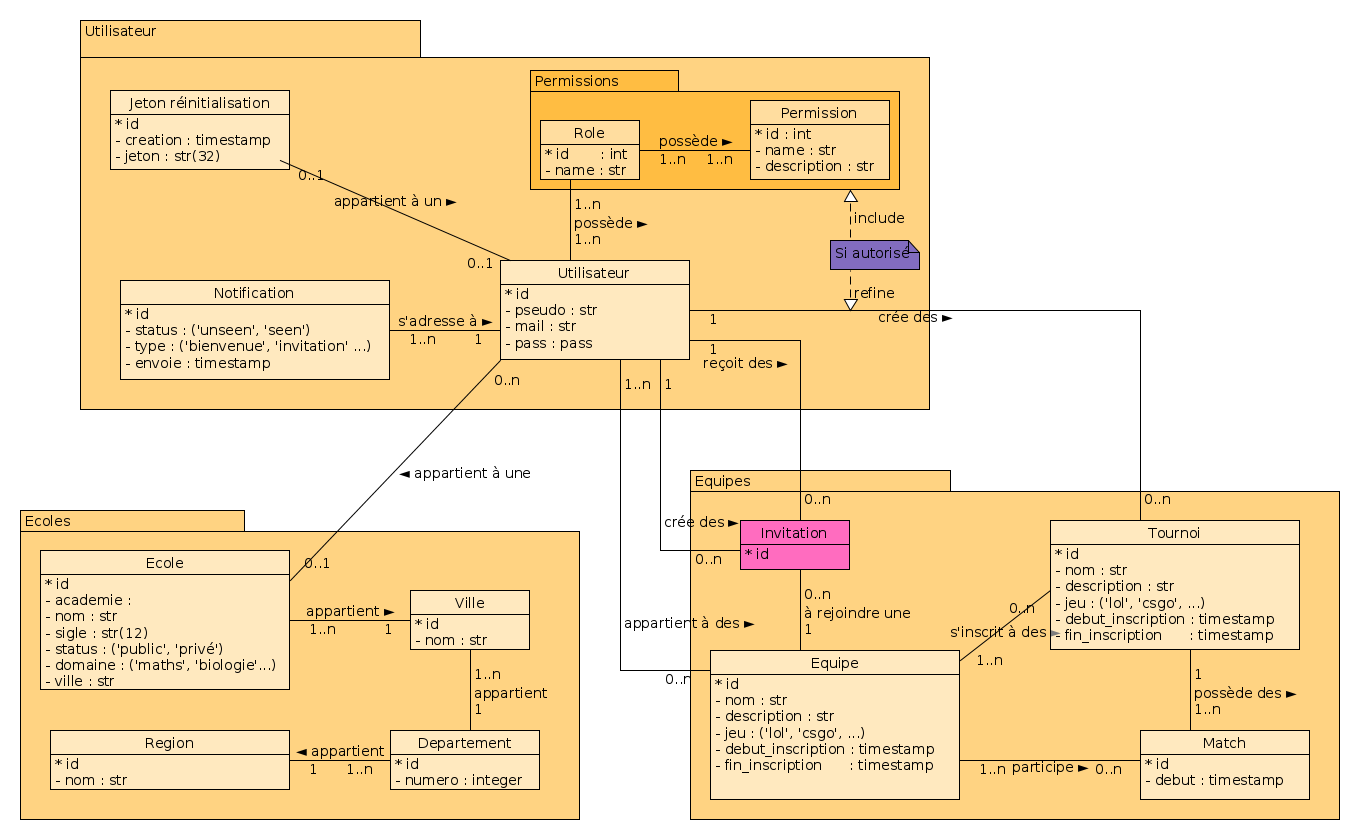
\includegraphics[width=17.5cm,keepaspectratio]{./images/uml.png}
	\end{center}
	\caption{\textit{Schéma UML de la base de données}}
	\label{uml}
      \end{figure}
      
      \newpage
      \subsubsection{Utilisateur}
	\paragraph{Permission} Représente une permission ponctuelle (créer une équipe, créer un tournoi, bannir un joueur, inscrire son équipe...)
	\paragraph{Rôle} Représente une ensemble de permissions (administrateur: toutes les permissions, modérateur: bannir un joueur, ...).
	\paragraph{Utilisateur} Possèdent différents rôles, et donc toutes les permissions liées aux rôles.
	Contient les informations relative à un utilisateur enregistré sur le site: mail, pseudo, mot de passe...
	
	Le mot de passe est hashé à l'aide de la fonction PHP 'password\_hash'.
	On protège ainsi efficacement l'accès par un tier au compte de l'utilisateur.
	(les détails techniques ne seront pas présentés ici, voir documentation \ref{password_hash} et \ref{password_salt})
	
	\paragraph{Notification} Un message destiné à attirer l'attention de l'utilisateur du site (e.x: le notifie d'une invitation à rejoindre une équipe)
	\paragraph{Jeton de réinitialisation} Une chaîne de 32 caractères générées aléatoirement.
	Ce jeton est généré et envoyé par mail à un utilisateur s'il a oublié son mot de passe.
	Il a alors 15 minutes pour changer son mot de passe en accédant au service consacré à cet effet.
      
      \subsubsection{Ecoles}
	Une base de données a été généré à partir de la page Wikipédia \ref{ecole_ingé}.
	Les données ont été extraite de la page, au format csv, à l'aide d'un programme Python (et de la bibliothèque BeautifulSoup \ref{beautifulsoup}).
	
	Cette base de donnée aura 2 utilités principales : auto-complétion pour la recherche, et organisation de tournois par région.
	Elle permettra également d'avoir des statistiques par région (fait t'on plus d'e-sport à Angers ou bien à Paris).
	
      \subsubsection{Equipes}
	\paragraph{Equipe}
	\paragraph{Tournoi}
	\paragraph{Match}
	\paragraph{Invitation}

      \subsubsection{API 'REST'}
	Une API a été implementé sur le modèle REST.
	
	La documentation a été généré via Doxygen, et est accessible à l'adresse \href{http://localhost:8080/doc/html/files.html}{\textit{http://localhost:8080/doc/html/files.html}}.
	
	Cependant, elle ne peut pas être entièrement considéré comme totalement 'REST', car le serveur enregistre des informations dans la session PHP,
	ce qui entre en contradiction avec le principe \ref{api_rest_session}. La satisfaction d'autres principes du 'REST' est également sujet à débat.
	
	Mais elle reste pratique et ouverte. Le client doit seulement récupéré le cookie 'PHP\_SESSID' via le service '/user/account/connect'.
	
      \begin{figure}[H]
	\begin{center}
	  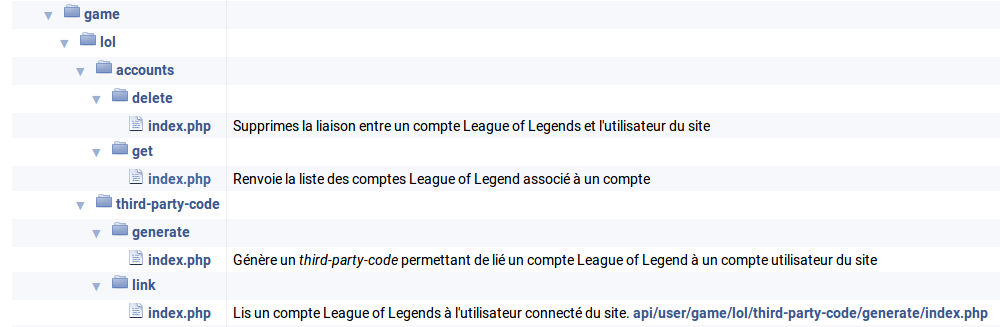
\includegraphics[width=14cm,keepaspectratio]{./images/api.png}
	\end{center}
	\caption{\textit{Partie de la page d'accueil de la documentation}}
	\label{api}
      \end{figure}
      
      \begin{figure}[H]
	\begin{center}
	  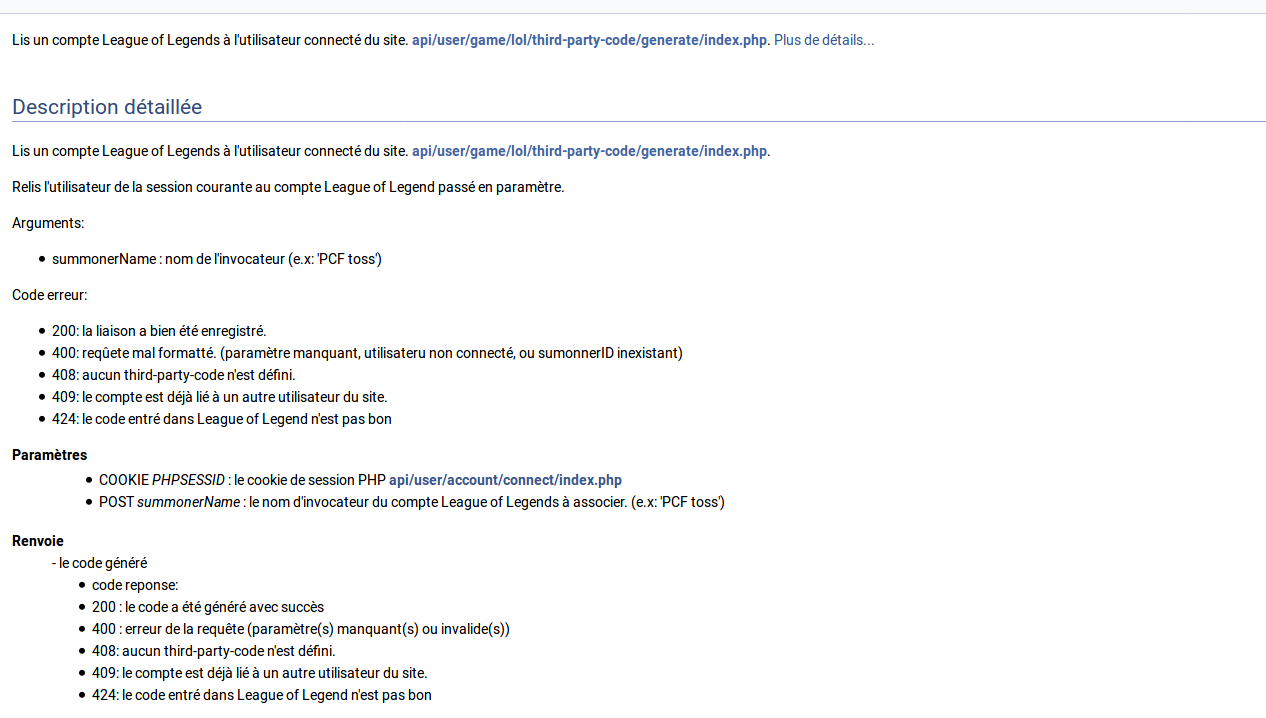
\includegraphics[width=14cm,keepaspectratio]{./images/link_account.png}
	\end{center}
	\caption{\textit{Détail d'une requête (lié un compte Lol à l'utilisateur du site)}}
	\label{link_account}
      \end{figure}

    \subsection{Front-end}
      \begin{figure}[H]
	\begin{center}
	  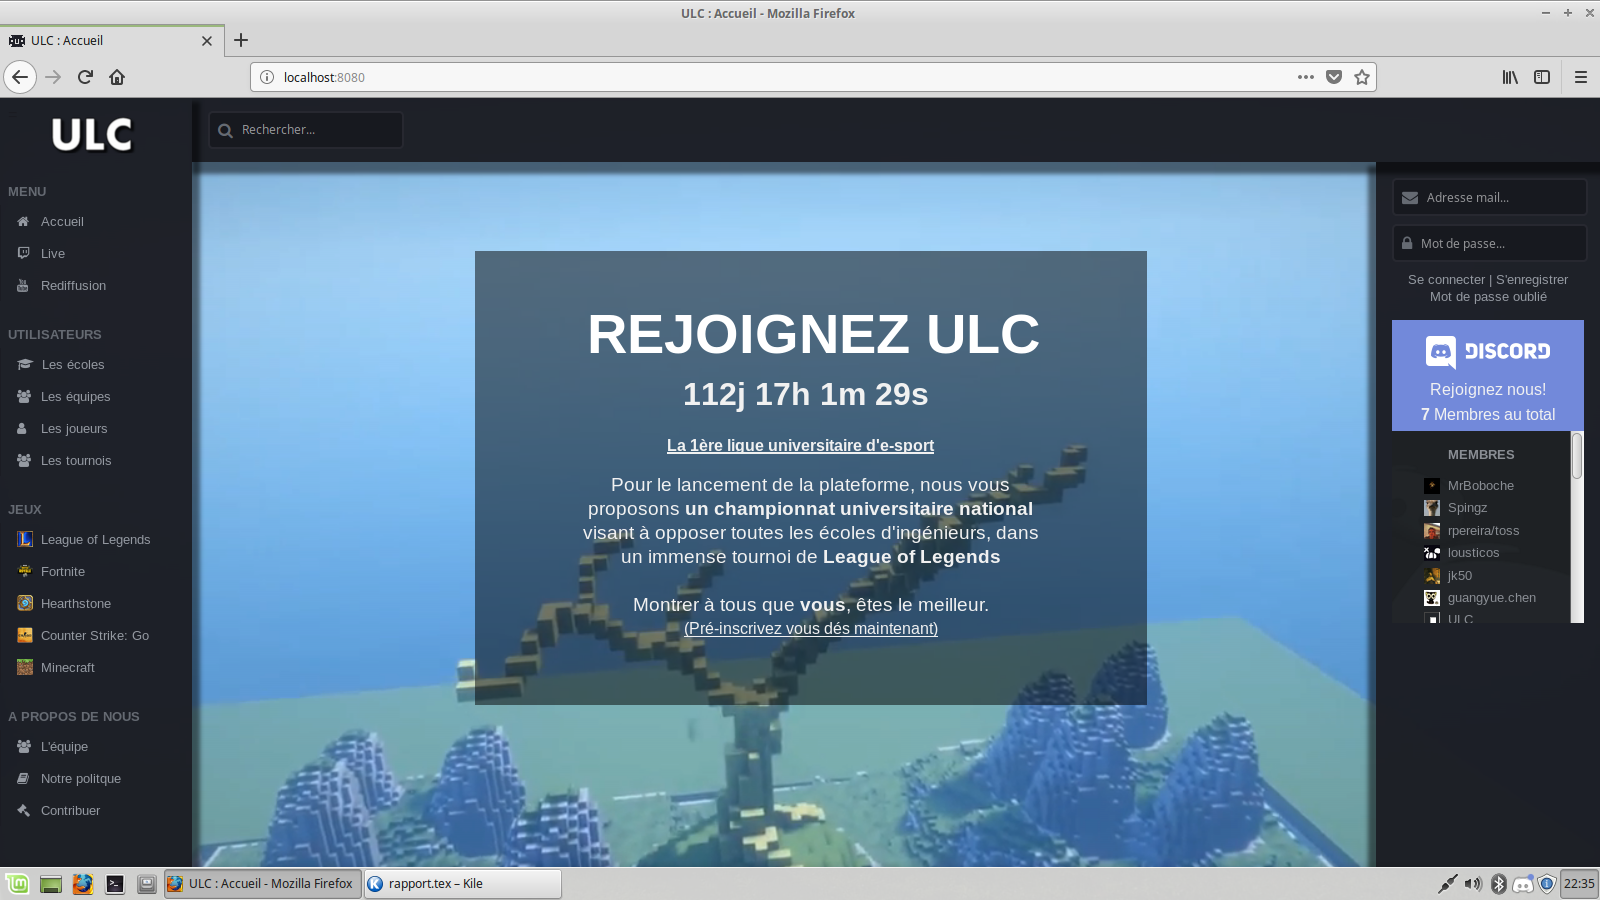
\includegraphics[width=16cm,keepaspectratio]{./images/site.png}
	\end{center}
	\caption{\textit{Page d'accueil du site}}
	\label{uml}
      \end{figure}
  
  \newpage
  \section{Conclusion}
  \newpage
  \section{Références}
  \begin{thebibliography}{}
    
    \bibitem{phpgoodpratices}\label{phpgoodpratices}
    'PHP The Right Way' - \href{https://github.com/codeguy/php-the-right-way/graphs/contributors}{\textit{+200 authors}} \newline
    \href{http://www.phptherightway.com/}{\textit{http://www.phptherightway.com/}}
    
    \bibitem{riotapi}\label{riotapi}
    API officiel de Riot Games \newline
    \href{https://developer.riotgames.com/}{\textit{https://developer.riotgames.com/}}
    
    \bibitem{discordapi}\label{discordapi}
    API officiel de Discord \newline
    \href{https://discordapp.com/developers/docs/intro}{\textit{https://discordapp.com/developers/docs/intro}}
    
    \bibitem{password_hash}\label{password_hash}
    php.net - password\_hash documentation \newline
    \href{http://php.net/manual/fr/function.password-hash.php}{\textit{http://php.net/manual/fr/function.password-hash.php}}
    
    \bibitem{password_salt}\label{password_salt}
    Salage de mot de passe \newline
    \href{https://en.wikipedia.org/wiki/Salt_(cryptography)}{\textit{https://en.wikipedia.org/wiki/Salt\_(cryptography)}}
    
    \bibitem{ecole_ingé}\label{ecole_ingé}
    Liste écoles d'ingénieur en France - Wikipédia \newline
    \href{https://fr.wikipedia.org/wiki/Liste_des_écoles_d'ingénieurs_en_France#Liste_des_207_écoles_françaises_accréditées_au_1er_septembre_2017}{\textit{https://fr.wikipedia.org/wiki/Liste\_des\_écoles\_d'ingénieurs\_en\_France}}
    
    \bibitem{beautifulsoup}\label{beautifulsoup}
    BeautifulSoup - Documentation\newline
    \href{https://www.crummy.com/software/BeautifulSoup/bs4/doc/}{\textit{https://www.crummy.com/software/BeautifulSoup/bs4/doc/}}
    
    \bibitem{api_rest_session}\label{api_rest_session}
    API REST - Wikipédia \newline
    \href{https://fr.wikipedia.org/wiki/Representational_state_transfer#Sans_état}{\textit{https://fr.wikipedia.org/wiki/Representational\_state\_transfer\#Sans\_état}}
    
  \end{thebibliography}
  
\end{document}
